\documentclass[13.5pt,aspecratio=169, xcolor=dvipsnames]{beamer}
\usepackage{graphicx} % Required for inserting images
\usepackage{subcaption}
\usepackage{amsfonts}
\usepackage{amsmath}
\usepackage{amssymb}
\usepackage{physics}
\usepackage{bm}
\usepackage{physics}
\usepackage{booktabs}
\usepackage{setspace}
\usepackage{xcolor}
\usepackage{wrapfig,lipsum}
\usepackage{etoolbox}
\usepackage{tikz}
\usepackage{multirow}
\usepackage{verbatim}
\usepackage{pifont}
\usepackage[most]{tcolorbox}
\usetheme{Madrid}
\useinnertheme{circles}

\DeclareMathOperator*{\argmax}{arg\,max}
\DeclareMathOperator*{\argmin}{arg\,min}
\graphicspath{{Images/}{./}} 
\usetheme{Copenhagen}
\definecolor{UBCblue}{rgb}{0.04706, 0.13725, 0.26667} 
\usecolortheme[named=UBCblue]{structure}
%\usecolortheme{beaver}
% \titlegraphic{\centering \LARGE MultiVerS}
\title{Improving scientific claim verification with
weak supervision and full-document context}
\author[CS431]{
    \begin{tabular}{c}
        \textbf{CS431.O12.KHCL} \\
        \textit{Instructor: Nguyen Duy Khanh} \\
        \bigskip
        \textbf{Group 13} \\
        Le Gia Khang \quad Nguyen Hoang Tan \quad Le Duy Khang
    \end{tabular}
}
\date{\today}
\definecolor{mylightgreencolor}{RGB}{144, 238, 144}
\definecolor{mylightredcolor}{RGB}{255, 204, 203}
\definecolor{mylightbluecolor}{RGB}{173,216,230}
\definecolor{blockbackgroundcolor}{RGB}{235,235,235}
\definecolor{blockbordercolor}{RGB}{79,79,79}

\setbeamertemplate{navigation symbols}{}
\setbeamertemplate{headline}{}
\setbeamercolor{huge text}{fg=white}
\setbeamertemplate{footline}{
    \leavevmode%
    \hbox{%
        \begin{beamercolorbox}[wd=.1\paperwidth,ht=2.25ex,dp=1ex,center]{author in head/foot}%
            \usebeamerfont{author in head/foot}\insertshortauthor
        \end{beamercolorbox}%
        \begin{beamercolorbox}[wd=.8\paperwidth,ht=2.25ex,dp=1ex,center]{title in head/foot}%
            \usebeamerfont{title in head/foot}\centering \insertshorttitle
        \end{beamercolorbox}%
        \begin{beamercolorbox}[wd=.1\paperwidth,ht=2.25ex,dp=1ex,right]{date in head/foot}%
            \insertframenumber{} / \inserttotalframenumber\hspace*{2ex} 
        \end{beamercolorbox}%
    }%
    \vskip0pt%
}
\setbeamertemplate{section in toc}{%
  \tikz[baseline=(tocseclabel.base)]{
    \node[fill=structure.fg,rounded corners,inner sep=4pt, font=\large\bfseries] (tocseclabel) {\color{white}\inserttocsectionnumber};
  }\hspace{0.5em}\large\bfseries\inserttocsection\vspace{0.3em}}


  \newtcolorbox{mybox}{
  colback=blockbackgroundcolor, % Background color (adjust as needed)
  colframe=blockbordercolor, % Frame color (adjust as needed)
  rounded corners,
  boxrule=0.2mm, % Frame width
  arc=2mm, % Radius of the rounded corners
  drop shadow, % Add a drop shadow (optional)
%   width=\tcboxwidth, % Adjust the width
%   hbox,
}




\newcommand{\raisedtext}[1]{%
  \raisebox{-0.2ex}{#1}%
}
  
\begin{document}
\begin{frame}
    \begin{picture}(0,0)
        \put(170,0){\makebox(0,0){\huge \textbf{\textcolor{UBCblue}{MultiVerS}}}}
    \end{picture}
    \maketitle
\end{frame}

% \begin{frame}
% 	\frametitle{Table of Contents} % Slide title, remove this command for no title
% 	\tableofcontents[subsectionstyle=hide]
% \end{frame}
%-------------------------------------------------------------------%


% \begin{frame}
%     \doublespacing
%         \frametitle{Presentation Overview} % Slide title, remove this command for no title
        
%         \tableofcontents % Output the table of contents (all sections on one slide)
%         %\tableofcontents[pausesections] % Output the table of contents (break sections up across separate slides)
% \end{frame}
    
%     %----------------------------------------------------------------------------------------
%     %	PRESENTATION BODY SLIDES
%     %----------------------------------------------------------------------------------------
    
%     \section{Lexical Semantics} % Sections are added in order to organize your presentation into discrete blocks, all sections and subsections are automatically output to the table of contents as an overview of the talk but NOT output in the presentation as separate slides
%     %------------------------------------------------
%     \begin{frame}
%         \doublespacing
%             \frametitle{Presentation Overview} % Slide title, remove this command for no title
            
%             \tableofcontents[currentsection] % Output the table of contents (all sections on one slide)
%             %\tableofcontents[pausesections] % Output the table of contents (break sections up across separate slides)
%     \end{frame}

% %-------------------------------------------------------------------%

\begin{frame}
    \onehalfspacing
    \frametitle{Task}
    \textbf{Definition of scientific claim verification from the S\raisedtext{CI}F\raisedtext{ACT} task:}
    \vspace*{-1em} 
    \begin{mybox}
            Given a claim $c$ and a \textit{candidate abstract} $a$. \\
            Label $y(c,a) \in \{SUPPORTS, REFUTES, NEI\}.$ \\
            Identify rationales $R(c, a) = \{r_1(c, a),......,r_n(c, a)\}.$
      \end{mybox}

      \begin{minipage}{0.45\textwidth}
        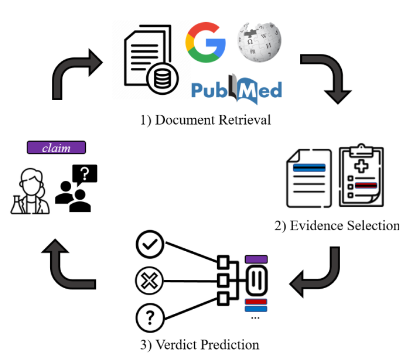
\includegraphics[width=\textwidth]{Task_Definition.png}
      \end{minipage}
      \begin{minipage}{0.45\textwidth}
        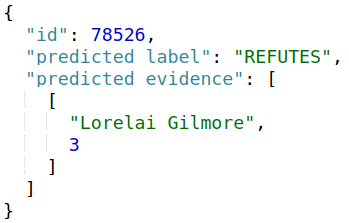
\includegraphics[width=\textwidth]{Json_data.png}
      \end{minipage}
\end{frame}
    
%--------------------------------------------------



\begin{frame}
    \onehalfspacing
    \frametitle{Task}
    \begin{minipage}{0.47\textwidth}
        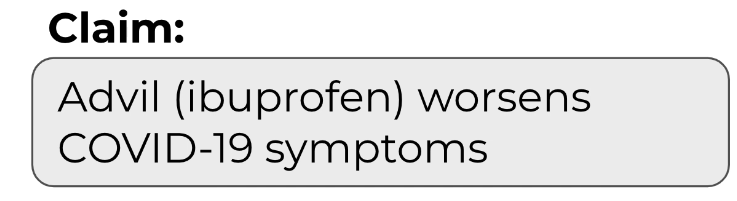
\includegraphics[width=\textwidth]{Claim.png}
        \visible<2-5> {
            \centering
            \begin{minipage}{0.7\textwidth}
            {\setbeamercolor{block body}{bg=Maroon}
            \begin{block}{}
                \begin{center}
                    \textbf{\textcolor{white}{Label: Refuted}}
                \end{center}
            \end{block}
            }
            \end{minipage}     
        }
        
        \bigskip
        \visible<3-5> {
            \begin{flushleft}
            Task Outputs
            \begin{enumerate}
                \item Fact-checking label
                \visible<4-> {\item Rationales justifying the label}
            \end{enumerate}
            \end{flushleft}
        }

    \end{minipage}
    \begin{minipage}{0.45\textwidth}
        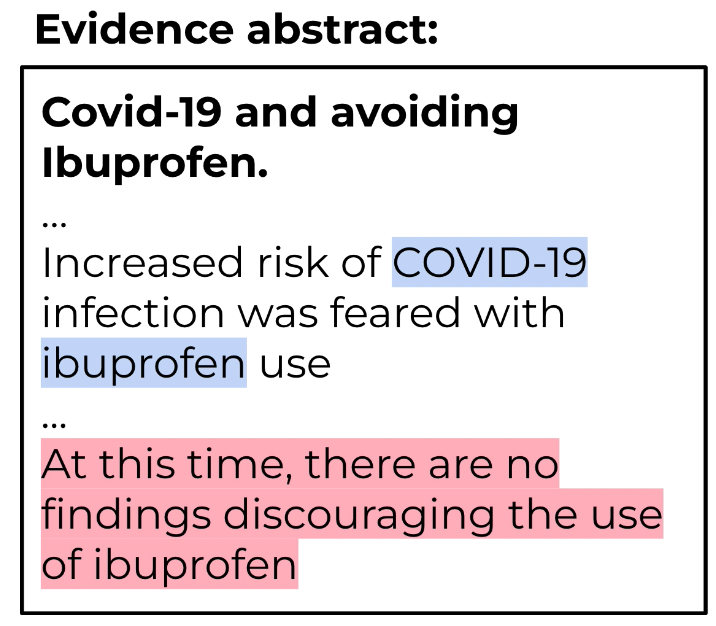
\includegraphics[width=1.2\textwidth]{Evidence_abstract.png}
        
        \visible<4-5> {
            \setbeamercolor{block body}{bg=mylightredcolor}
            \vspace*{-2.5em}
            \hspace{9em}
            \begin{minipage}{0.4\textwidth}
            \begin{block}{}
                \begin{center}
                    \textbf{\textcolor{black}{Rationale}}
                \end{center}
            \end{block}
         \end{minipage}     
        }

        \visible<5> {
            \setbeamercolor{block body}{bg=mylightbluecolor}
            \vspace*{-8em}
            \hspace{9em}
            \begin{minipage}{0.5\textwidth}
            \begin{block}{}
                \begin{center}
                    {\textcolor{black}{Context required}}
                \end{center}
            \end{block}
         \end{minipage}     
        }
    \end{minipage}
\end{frame}
    
%--------------------------------------------------

    \begin{frame}
    \onehalfspacing
        \frametitle{Prior work: Extract-then-label}
        \only <1> {
            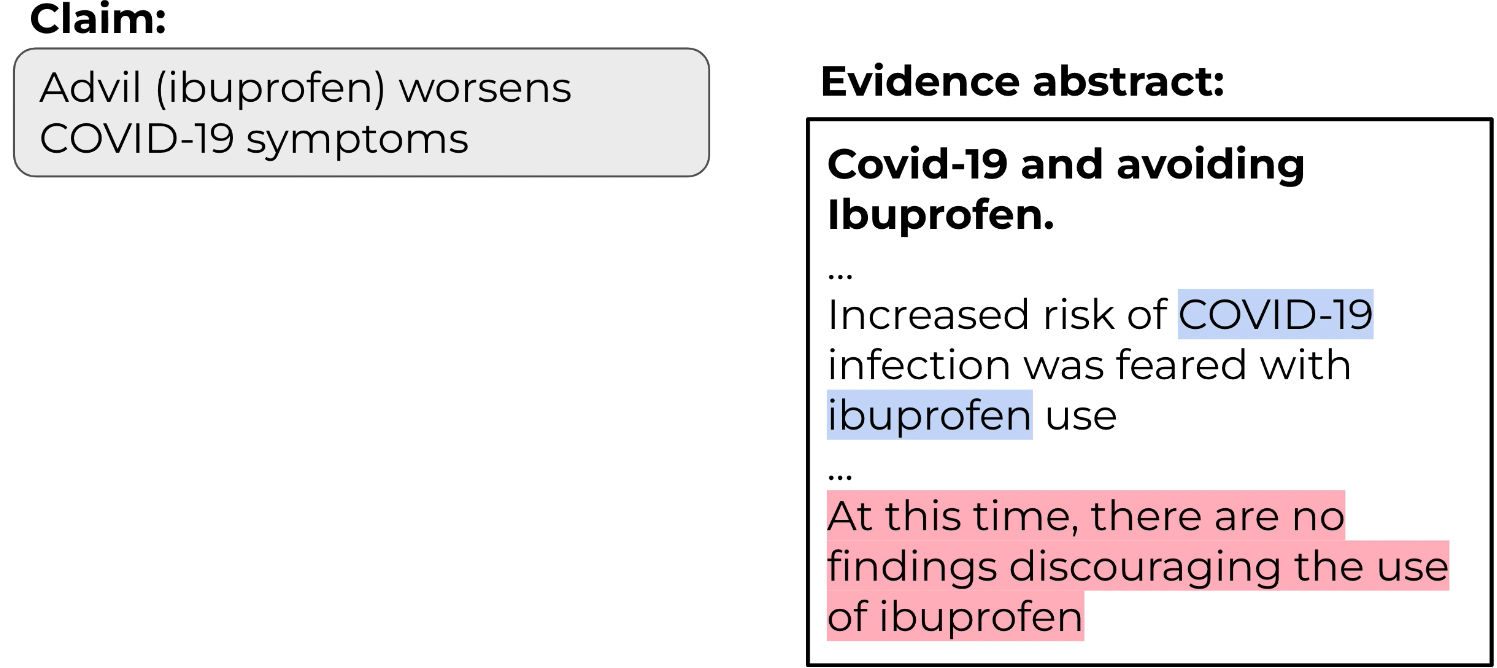
\includegraphics[width=\textwidth]{Extract_then_label_1.png}
        }
        \only <2-> {
            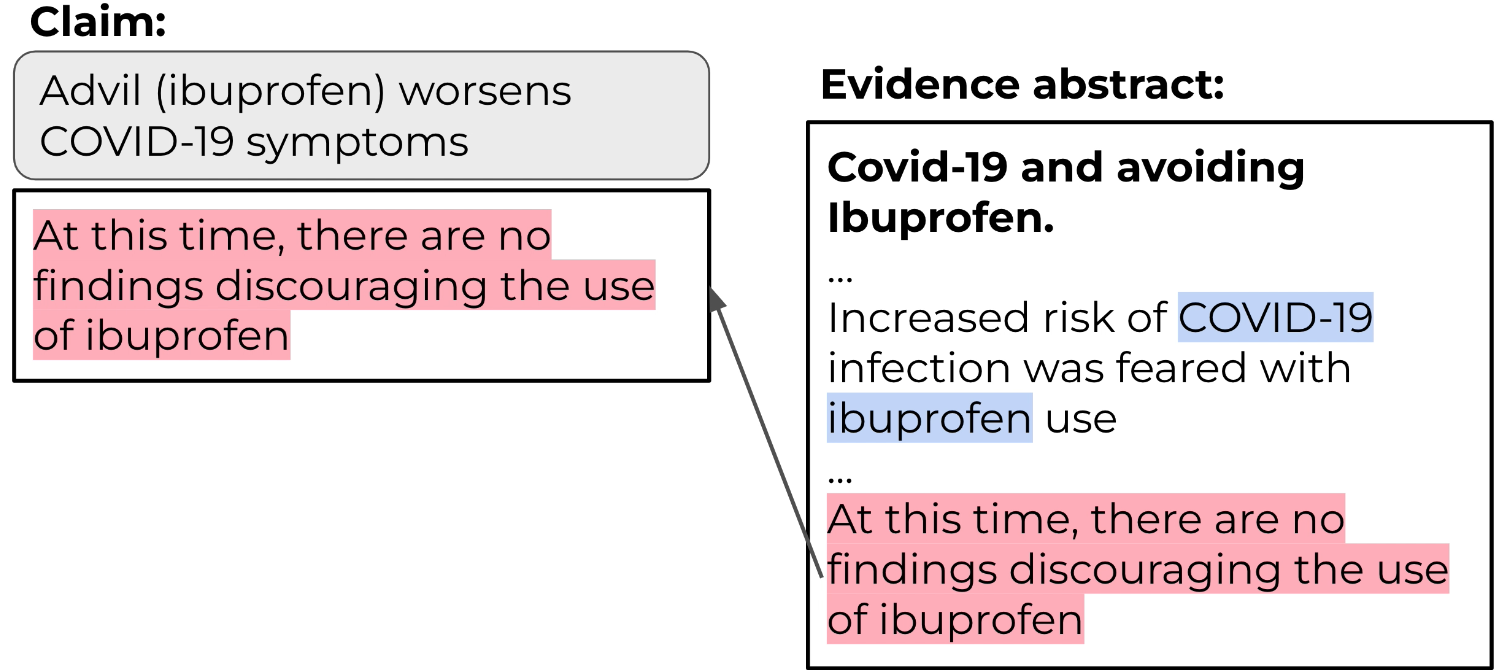
\includegraphics[width=\textwidth]{Extract_then_label_2.png}
        }

        \only <3-> {
            \vspace*{-7em}
            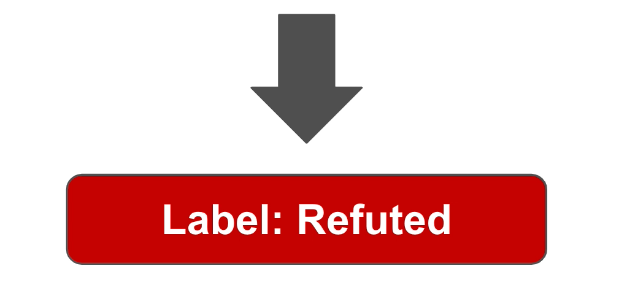
\includegraphics[width=0.5\textwidth]{produce_label.png}
        }

        \only <4> {
            \begin{overlayarea}{\textwidth}{\textheight}
                \vspace*{-3.5em}
                \hspace*{17em}
                \begin{minipage}{0.45\textwidth}
                    \begin{block}{Drawbacks of extract-then-label:}
                        \begin{enumerate}
                            \item Rationales may lack context
                            \item Requires rationale supervision during training
                        \end{enumerate}
                    \end{block}
                \end{minipage}
            \end{overlayarea}
        }
    \end{frame}
    
    
    %------------------------------------------------

    \begin{frame}
        \onehalfspacing
        \frametitle{Prior models}

        \begin{minipage}{0.6\textwidth}
            \begin{block}{}
                Given a claim $c$ and candidate abstract $a$
            \end{block}
        \end{minipage}

        \bigskip
        
        \textbf{These models make predictions in 2 steps:}
        \vspace*{-1em} 
        \begin{mybox}
            Predict rationales $ \hat{R}(c,a) = \{ \hat{r_1}(c,a),... \hat{r_n}(c,a)\}$ \\
            Then, make a label prediction $\hat{y}(c, f_R(\hat{R}(c,a)))$
          \end{mybox}
    
    \end{frame}
        
    %--------------------------------------------------
    
    \begin{frame}
        \onehalfspacing
        \frametitle{MultiVerS}
        \begin{block}{A multitask system for full-context scientific claim verification}
            \begin{itemize}
                \item Predict $\hat{y}(c, a)$ directly based on an encoding of the entire claim and abstract.
                \item Enforce consistency of $\hat{R}(c, a)$ with $\hat{y}(c; a)$ during decoding.
            \end{itemize}
        \end{block}
    \end{frame}
        
    %--------------------------------------------------

    \begin{frame}
        \onehalfspacing
        \frametitle{MultiVerS}
        \textbf{Long document encoding:}
        \vspace*{-1em} 
        \begin{mybox}
            A claim $c$ and candidate abstract $a$ consisting of title $t$ and sentences $s_1,...,s_n$. \\
            The $</s>$ token following each sentence $s_i$ is notated as $</s>_i$. 
          \end{mybox}

          \begin{figure}[h]
            \centering
            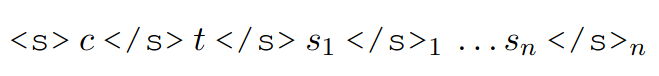
\includegraphics[width=0.8\textwidth]{Long_document_encoding.png}
          \end{figure}

          \begin{block}{}
            Global attention is assigned  to $<s>$ token, all tokens in $c$ and all $</s>$ tokens.
          \end{block}


    \end{frame}
        
    %--------------------------------------------------
    
    
    \begin{frame}
        \onehalfspacing
            \frametitle{MultiVerS}
            \only<1>{
                \begin{figure}[h]
                    \centering
                    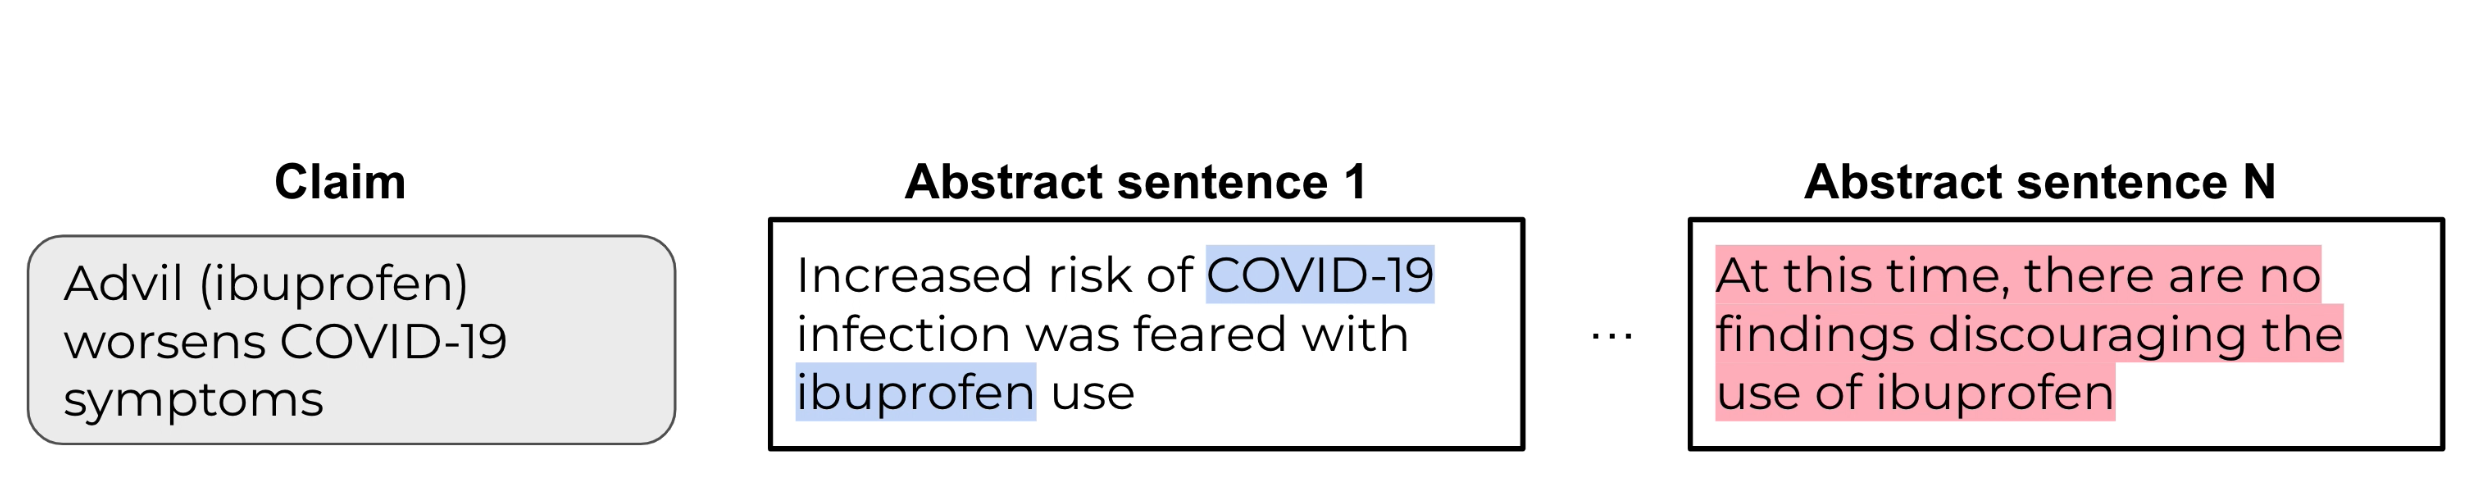
\includegraphics[width=\linewidth]{MultiVerS_1.png}
            \end{figure}
            }
            \only<2>{
                \begin{figure}[h]
                    \centering
                    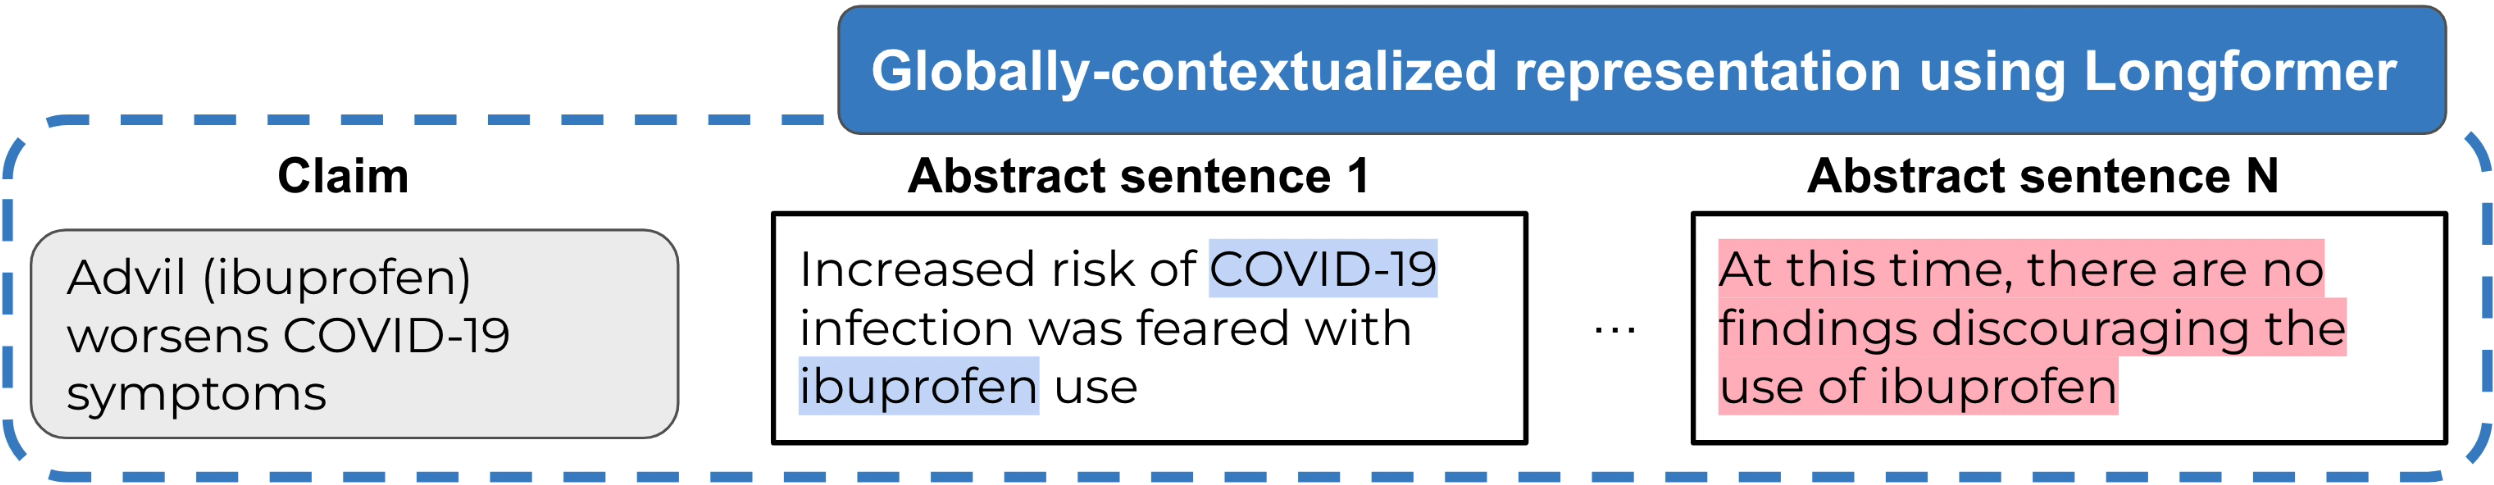
\includegraphics[width=\linewidth]{MultiVerS_2.png}
            \end{figure}
            }

            \only<3>{
                \begin{figure}[h]
                    \centering
                    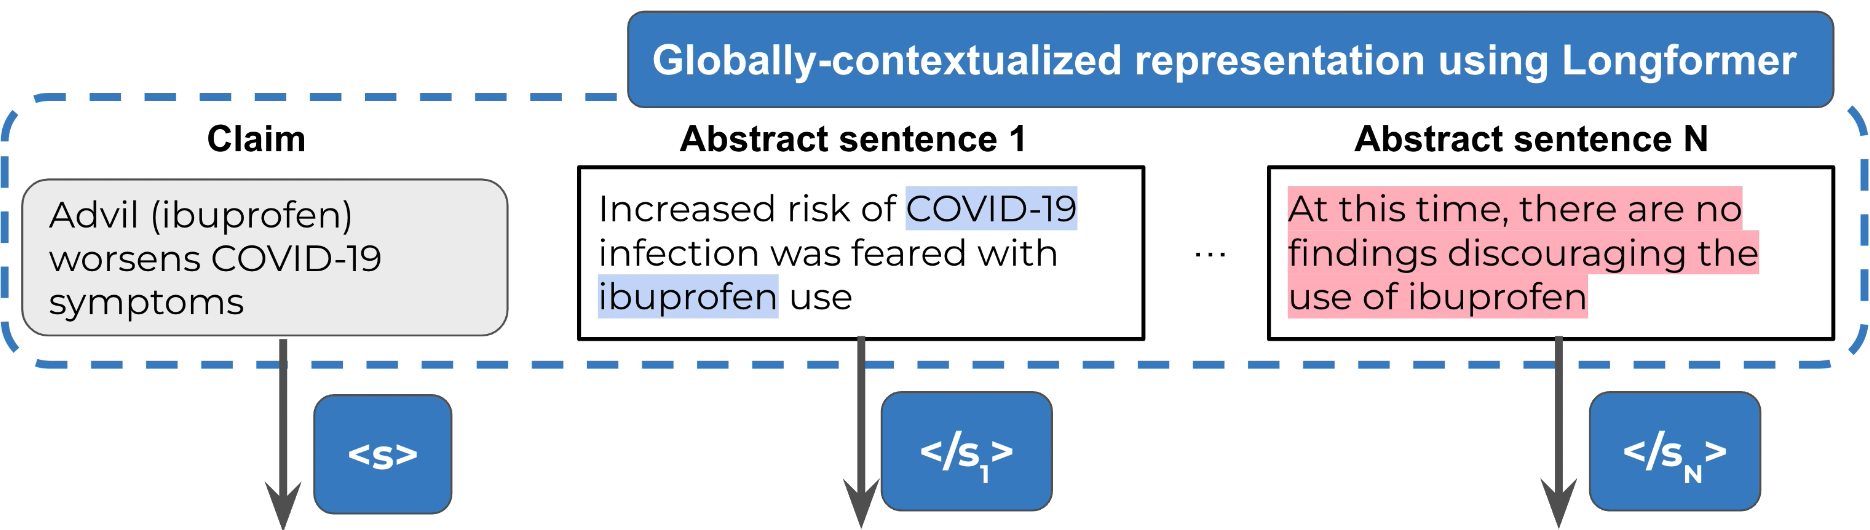
\includegraphics[width=\linewidth]{MultiVerS_3.png}
                    
            \end{figure}
            }

            \only<4->{
                \begin{figure}[h]
                    \centering
                    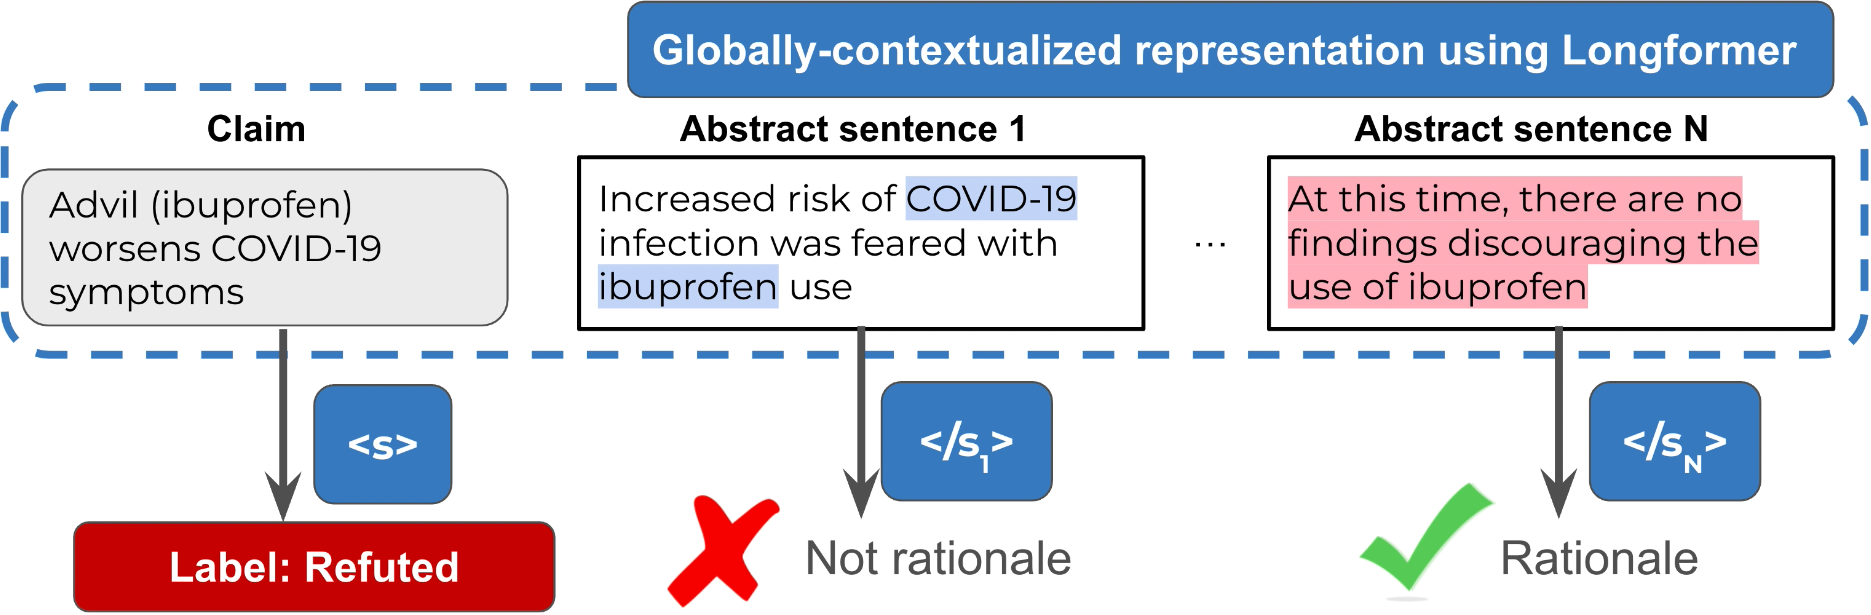
\includegraphics[width=\linewidth]{MultiVerS_4.png}
                \end{figure}
            }
            \only<5-> {
                 \begin{minipage}{0.52\textwidth}
                    {\Large
                    \begin{tcolorbox}[ams align,colback=white]
                        \hspace{-0.75em} \mathcal{L} = \mathcal{L}_{label} + \lambda_{rationale} \mathcal{L}_{rationale} \nonumber
                    \end{tcolorbox}
                    }
                \end{minipage}
                \hspace{0.2em}
                \begin{minipage}{0.45\textwidth}
                    \begin{block}{Benefits of multitask approach:}
                        \begin{enumerate}
                            \item Incorporates all relevant context
                            \item Can train on instances with no rationale annotations
                        \end{enumerate}
                    \end{block}
                \end{minipage}
            }
                
\end{frame}
    
%------------------------------------------------



\begin{frame}
    \onehalfspacing
        \frametitle{Experiments}
        \begin{table}[h]
            \centering
            \resizebox{\textwidth}{!}{
            \begin{tabular}{lllccccccc}
                \hline
                \textbf{Dataset} & \textbf{Domain} & \textbf{Claim source} & \textbf{Open} & \textbf{Has NEI}  & \textbf{Claim complexity} & \textbf{Negation method} & \textbf{Train claims} & \textbf{Eval claims} & \textbf{$> 512$
                tokens}\\
                \hline
                HealthVer & COVID & TREC-COVID & \ding{55} & \ding{51} & Complex & Natural & 1,622 & 230 & 14.9\% \\
                COVIDFact & COVID & Reddit & \ding{55} & \ding{55} & Complex & Automatic & 903 & 313 & 12.4\% \\ 
                S\raisedtext{CI}F\raisedtext{ACT} & Biomed & Citations & \ding{51} & \ding{51} & Atomic & Human & 1,109 & 300 & 27.4\% \\
                \hline
                F\raisedtext{EVER} & Wiki & Wikipedia & - & \ding{51} & Atomic & Human & 130,644 & - & 33.2\% \\
                P\raisedtext{UBMED}QA & Biomed & Paper titles & - & \ding{51} & Complex & Automatic & 58,370 & - & 12.1\% \\
                E\raisedtext{VIDENCE}I\raisedtext{NFERENCE} & Biomed & ICO prompts & - & \ding{51} & Atomic & Automatic & 7,395 & - & 42.7\% \\
            \end{tabular}
            }
            \caption{Summary of datasets used in experiments }
        \end{table}
        


\end{frame}
%------------------------------------------------
    
\begin{frame}
\onehalfspacing
    \frametitle{Experiments}
    \begin{minipage}{0.3\textwidth}
        \textbf{Target datasets:}
        \begin{itemize}
            \item HealthVer
            \item COVID-Fact
            \item SciFact
        \end{itemize}
    \end{minipage}
    \begin{minipage}{0.69\textwidth}
        \visible <2-> {
        \begin{minipage}{0.75\textwidth}
            \begin{block}{}
                \hspace{0.5em} Roughly 1000 claims / dataset. \\
                \hspace{0.5em} Expert annotations are expensive
            \end{block}
        \end{minipage} 
        }
    \end{minipage}

    \bigskip
    \visible<3-> {
        \textbf{Traning procedure:}
        \begin{itemize}
            \item \textbf{Stage 1:} Train on a combination of \textit{labeled out of domain} data \textit{weakly-labeled in-domain data.}
            \item \textbf{Stage 2:} Continue training on data from each target dataset. 
        \end{itemize}
    }
    \bigskip
    \vspace*{-1em}
    \visible<4-> {
        \textbf{Domain adaptation settings:}
        \begin{itemize}
            \item \textbf{Zero-shot:} Stage 1 training only.
            \item \textbf{Few-shot:} 45 instances from target datasets.
            \item \textbf{Full-supervised:} All target data.
        \end{itemize}
    }



\end{frame}
%------------------------------------------------


\begin{frame}
    \onehalfspacing
        \frametitle{Data: Stage 1}
        \begin{minipage}[t]{0.42\textwidth}
            {
            \vspace*{-7em}
            \centering
            \textbf{Supervised} out-of-domain data (FEVER)

            

            \begin{block}{}
                LeBron James was born in \\ Ohio
            \end{block}
            {
            \setbeamercolor{block body}{bg=mylightgreencolor}

                \vspace*{-2em}
                \hspace{3em}
                \begin{minipage}{0.7\textwidth}

                \begin{block}{}
                    \centering
                    Label: Supported
                \end{block}
            \end{minipage}
            }

            \bigskip
            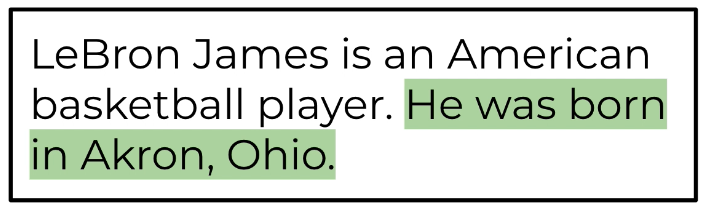
\includegraphics[width=\textwidth]{LeBron_James_claim.png}
            }
        \end{minipage}
        \hfill\vrule height 90pt width 2pt\hfill
        \begin{minipage}[t]{0.54\textwidth}
            {
            \vspace*{-7em}

            \only<1> {
                \phantom{
                \centering
                \textbf{Weakly-supervised} in-domain data
                fdjjnf
                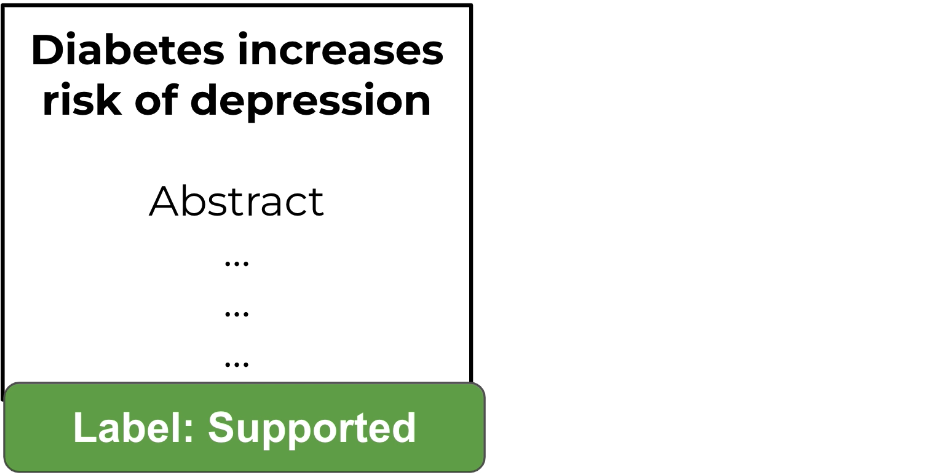
\includegraphics[width=\textwidth]{Stage_1_data_0.png} 
                }

            }

            \only<2-> {
                \centering
                \textbf{Weakly-supervised} in-domain data
                \phantom{                fdjjnf
                }
            }
            \only<2> {
                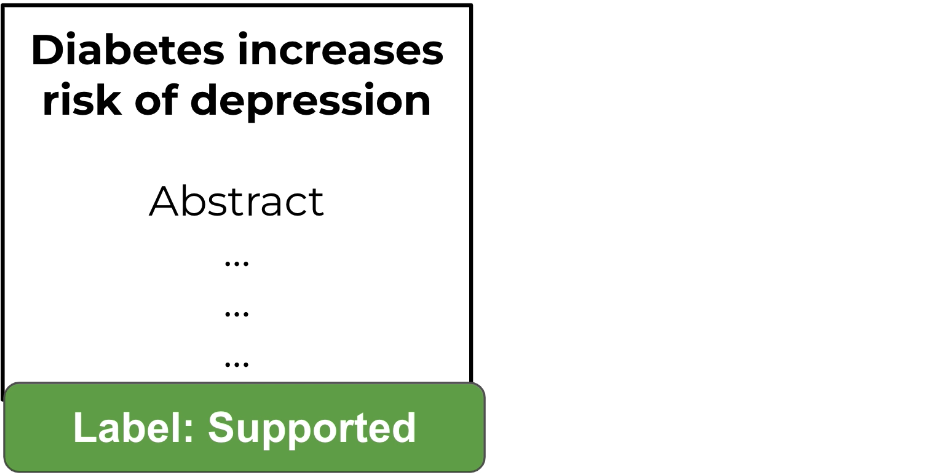
\includegraphics[width=\textwidth]{Stage_1_data_0.png}
            }

            \only<3> {
                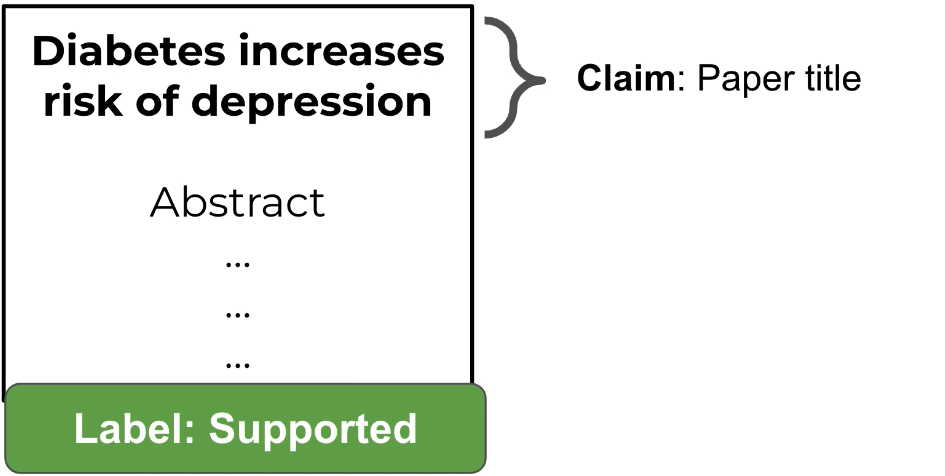
\includegraphics[width=\textwidth]{Stage_1_data_1.png}
            }

            \only<4-> {
                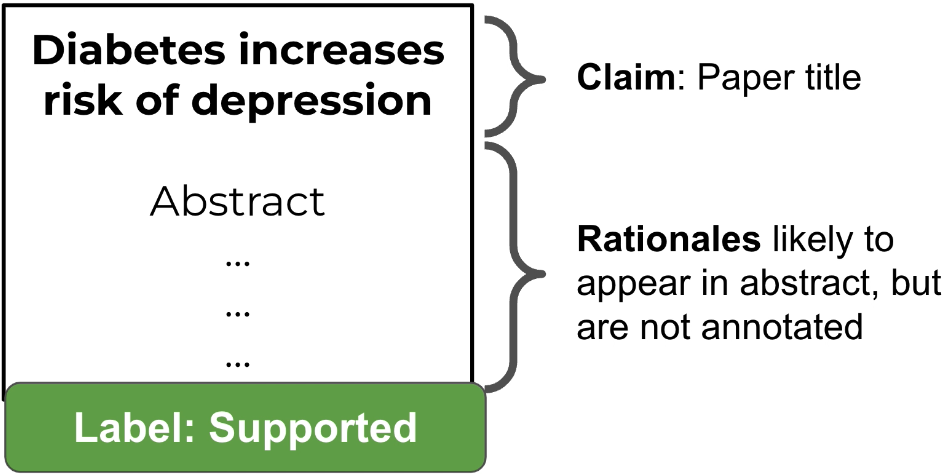
\includegraphics[width=\textwidth]{Stage_1_data_2.png}
            }

            \vspace*{-2em}
            \visible<5> {
                \begin{center}
                    \begin{minipage}{0.9\textwidth}
                        \begin{block}{}
                            MultiVerS can train on these examples, even though no rationale annotations are provided
                        \end{block}
                    \end{minipage}
                \end{center}
            }
            }
        \end{minipage}
       


    
    
\end{frame}
%------------------------------------------------

\begin{frame}
    \onehalfspacing
        \frametitle{Evaluation}
        \textbf{Abstract-level evaluation:}
        \vspace*{-1em} 
        \begin{mybox}
                \textbullet \hspace{0.3em} Identifying abstracts that SUPPORT or REFUTE each claim. \\
                \textbullet \hspace{0.3em} Predicting the correct label $y(c, a)$ is sufficient
        \end{mybox}

        \bigskip

        \textbf{Sentence-level evaluation:}
        \vspace*{-1em} 
        \begin{mybox}
                \textbullet \hspace{0.3em} It combines the accuracy of abstract-level label prediction with the precision of rationale identification.
        \end{mybox}

    
\end{frame}
%------------------------------------------------

\begin{frame}
    \onehalfspacing
        \frametitle{Evaluation}
        \begin{figure}[h]
            \centering
            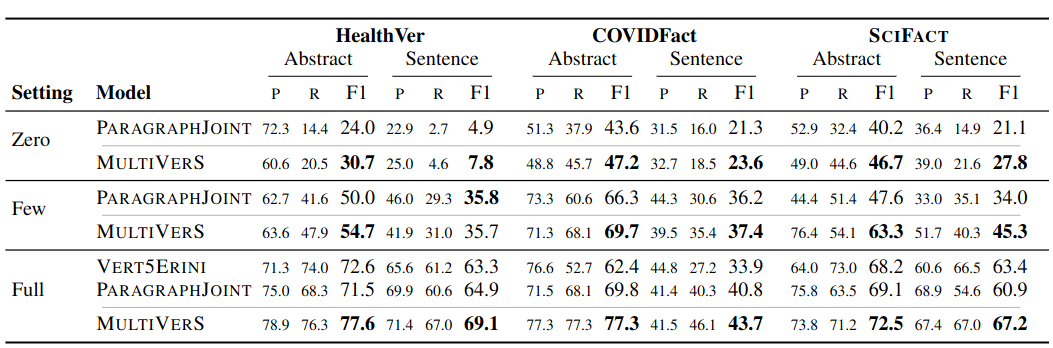
\includegraphics[width=\textwidth]{Results.png}
        \end{figure}
        \begin{center}
            Table 2: Performance of MultiVerS and baselines.
        \end{center}
    
\end{frame}
%------------------------------------------------
\begin{frame}[fragile]
    \onehalfspacing
        \frametitle{Our Reproduction Performance}
        \textbf{covidfact\_covidfact.jsonl:}
        \vspace*{-1em} 
        \begin{mybox}
        \begin{semiverbatim}
\{
    "abstract_label_only_precision": 0.7728706624605678,
    "abstract_label_only_recall": 0.7728706624605678,
    "abstract_label_only_f1": 0.7728706624605678,
    "sentence_label_precision": 0.41694915254237286,
    "sentence_label_recall": 0.458955223880597,
    "sentence_label_f1": 0.43694493783303723
\}\end{semiverbatim}
    \end{mybox}
\end{frame}

%------------------------------------------------


\begin{frame}[fragile]
    \onehalfspacing
        \frametitle{Our Reproduction Performance}
        \textbf{covidfact\_fever.jsonl:}
\vspace*{-1em} 
\begin{mybox}
\begin{semiverbatim}
\{
    "abstract_label_only_precision": 0.9583333333333334,
    "abstract_label_only_recall": 0.14511041009463724,
    "abstract_label_only_f1": 0.25205479452054796,
    "sentence_label_precision": 0.631578947368421,
    "sentence_label_recall": 0.04477611940298507,
    "sentence_label_f1": 0.08362369337979093
\}\end{semiverbatim}
\end{mybox}
\end{frame}
%------------------------------------------------



\begin{frame}[fragile]
    \onehalfspacing
        \frametitle{Our Reproduction Performance}
        \textbf{covidfact\_fever\_sci.jsonl:}
\vspace*{-1em} 
\begin{mybox}
\begin{semiverbatim}
\{
    "abstract_label_only_precision": 0.4882154882154882,
    "abstract_label_only_recall": 0.45741324921135645,
    "abstract_label_only_f1": 0.4723127035830619,
    "sentence_label_precision": 0.5444444444444444,
    "sentence_label_recall": 0.0914179104477612,
    "sentence_label_f1": 0.15654952076677317
\}\end{semiverbatim}
\end{mybox}
\end{frame}
%------------------------------------------------



\begin{frame}[fragile]
    \onehalfspacing
        \frametitle{Our Reproduction Performance}
        \textbf{healthver\_fever.jsonl:}
\vspace*{-1em} 
\begin{mybox}
\begin{semiverbatim}
\{
    "abstract_label_only_precision": 0.8,
    "abstract_label_only_recall": 0.00667779632721202,
    "abstract_label_only_f1": 0.013245033112582783,
    "sentence_label_precision": 1.0,
    "sentence_label_recall": 0.0027223230490018148,
    "sentence_label_f1": 0.005429864253393665
\}\end{semiverbatim}
\end{mybox}
\end{frame}
%------------------------------------------------

\begin{frame}[fragile]
    \onehalfspacing
        \frametitle{Our Reproduction Performance}
        \textbf{healthver\_fever\_sci.jsonl:}
\vspace*{-1em} 
\begin{mybox}
\begin{semiverbatim}
\{
    "abstract_label_only_precision": 0.6059113300492611,
    "abstract_label_only_recall": 0.20534223706176963,
    "abstract_label_only_f1": 0.30673316708229426,
    "sentence_label_precision": 0.40625,
    "sentence_label_recall": 0.011796733212341199,
    "sentence_label_f1": 0.022927689594356263
\}\end{semiverbatim}
\end{mybox}
\end{frame}
%------------------------------------------------

\begin{frame}[fragile]
    \onehalfspacing
        \frametitle{Our Reproduction Performance}
        \textbf{healthver\_healthver.jsonl:}
\vspace*{-1em} 
\begin{mybox}
\begin{semiverbatim}
\{
    "abstract_label_only_precision": 0.7892918825561313,
    "abstract_label_only_recall": 0.7629382303839732,
    "abstract_label_only_f1": 0.7758913412563666,
    "sentence_label_precision": 0.7194525904203324,
    "sentence_label_recall": 0.6678765880217786,
    "sentence_label_f1": 0.6927058823529412
\}\end{semiverbatim}
\end{mybox}
\end{frame}
%------------------------------------------------

\begin{frame}[fragile]
    \onehalfspacing
        \frametitle{Our Reproduction Performance}
        \textbf{scifact\_fever.jsonl:}
\vspace*{-1em} 
\begin{mybox}
\begin{semiverbatim}
\{
    "abstract_label_only_precision": 0.8378378378378378,
    "abstract_label_only_recall": 0.13963963963963963,
    "abstract_label_only_f1": 0.23938223938223935,
    "sentence_label_precision": 0.7307692307692307,
    "sentence_label_recall": 0.051351351351351354,
    "sentence_label_f1": 0.09595959595959597
\}\end{semiverbatim}
\end{mybox}
\end{frame}
%------------------------------------------------

\begin{frame}[fragile]
    \onehalfspacing
        \frametitle{Our Reproduction Performance}
        \textbf{scifact\_fever\_sci.jsonl:}
\vspace*{-1em} 
\begin{mybox}
\begin{semiverbatim}
\{
    "abstract_label_only_precision": 0.4900990099009901,
    "abstract_label_only_recall": 0.44594594594594594,
    "abstract_label_only_f1": 0.4669811320754717,
    "sentence_label_precision": 0.7017543859649122,
    "sentence_label_recall": 0.10810810810810811,
    "sentence_label_f1": 0.1873536299765808
\}\end{semiverbatim}
\end{mybox}
\end{frame}
%------------------------------------------------

\begin{frame}[fragile]
    \onehalfspacing
        \frametitle{Our Reproduction Performance}
        \textbf{scifact\_scifact.jsonl:}
\vspace*{-1em} 
\begin{mybox}
\begin{semiverbatim}
\{
    "abstract_label_only_precision": 0.7383177570093458,
    "abstract_label_only_recall": 0.7117117117117117,
    "abstract_label_only_f1": 0.7247706422018348,
    "sentence_label_precision": 0.6739130434782609,
    "sentence_label_recall": 0.6702702702702703,
    "sentence_label_f1": 0.6720867208672086
\}\end{semiverbatim}
\end{mybox}
\end{frame}
%------------------------------------------------


\begin{frame}
    \onehalfspacing
        \frametitle{Results}

        \only<1> {
            \vspace*{-2pt}
            \hspace{1pt}
            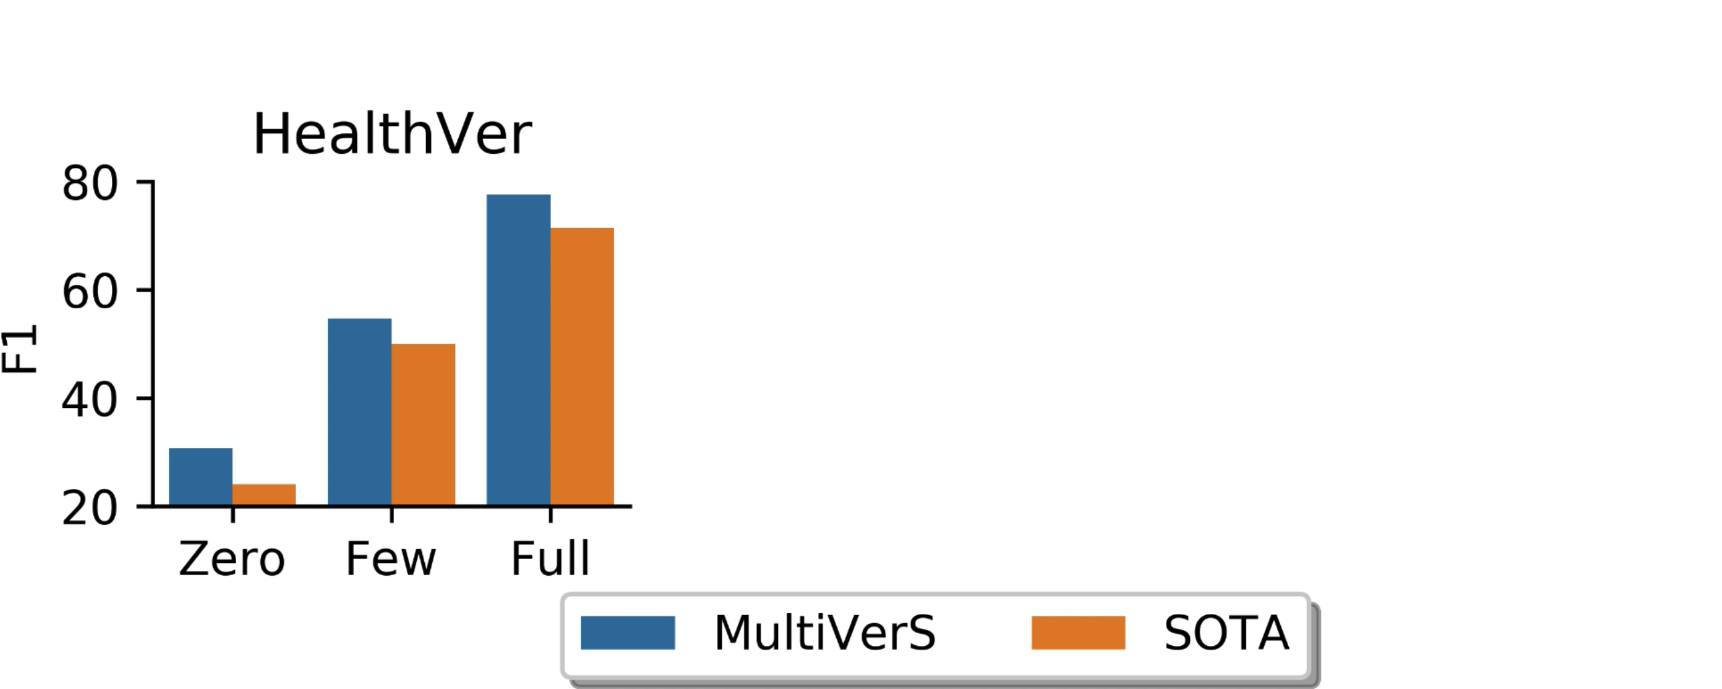
\includegraphics[width=\textwidth]{Result_0.png}

        }
        \only<2> {
            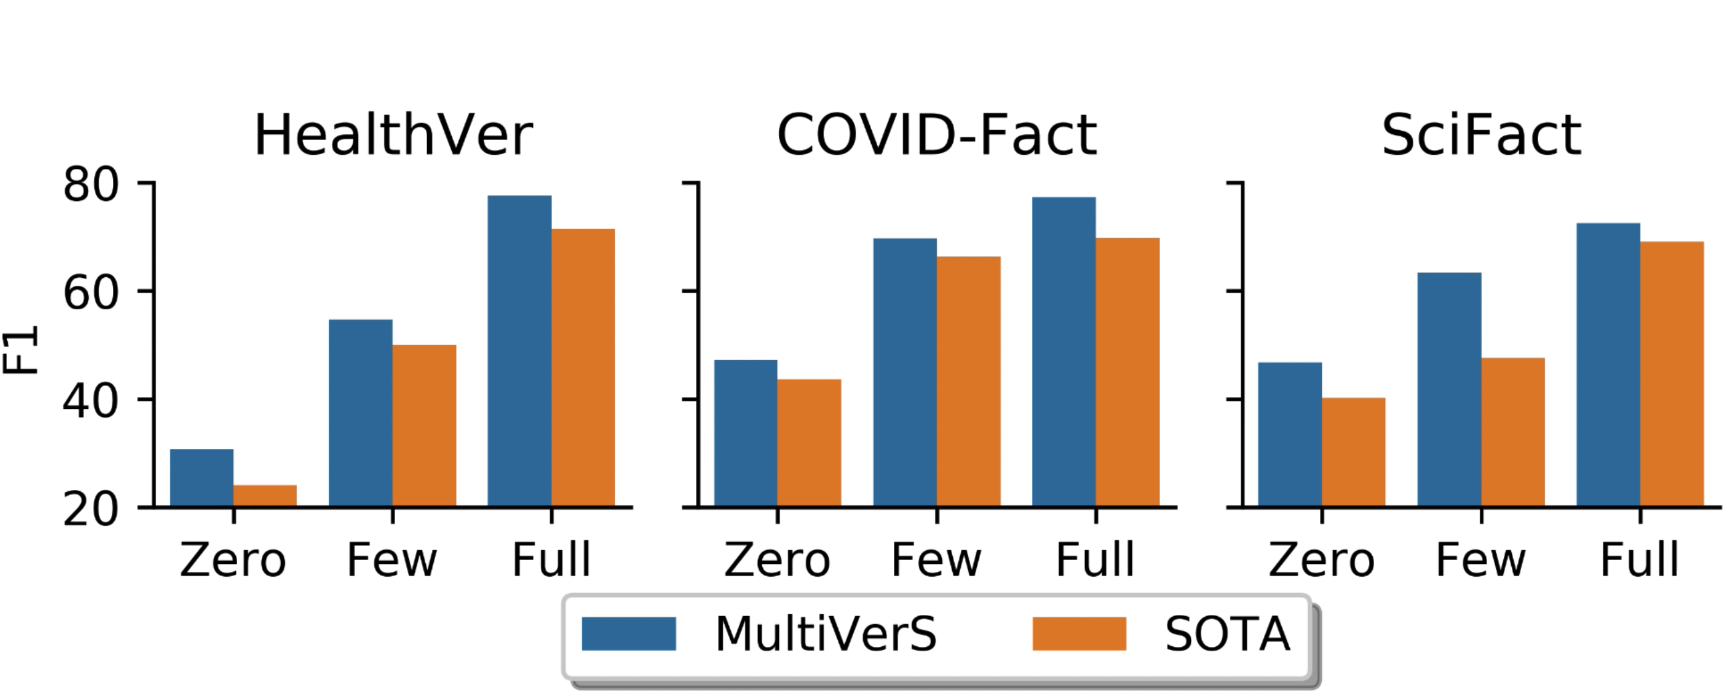
\includegraphics[width=\textwidth]{Result_1.png}

            \begin{minipage}{0.6\textwidth}
                \begin{block}{}
                    \vspace*{0.5em}MultiVerS outperforms SOTA on all datasets
                \end{block}
            \end{minipage}
        }
       

    
\end{frame}
%------------------------------------------------

\begin{frame}
    \onehalfspacing
        \frametitle{Ablations: Training strategy}

        \only<1> {
            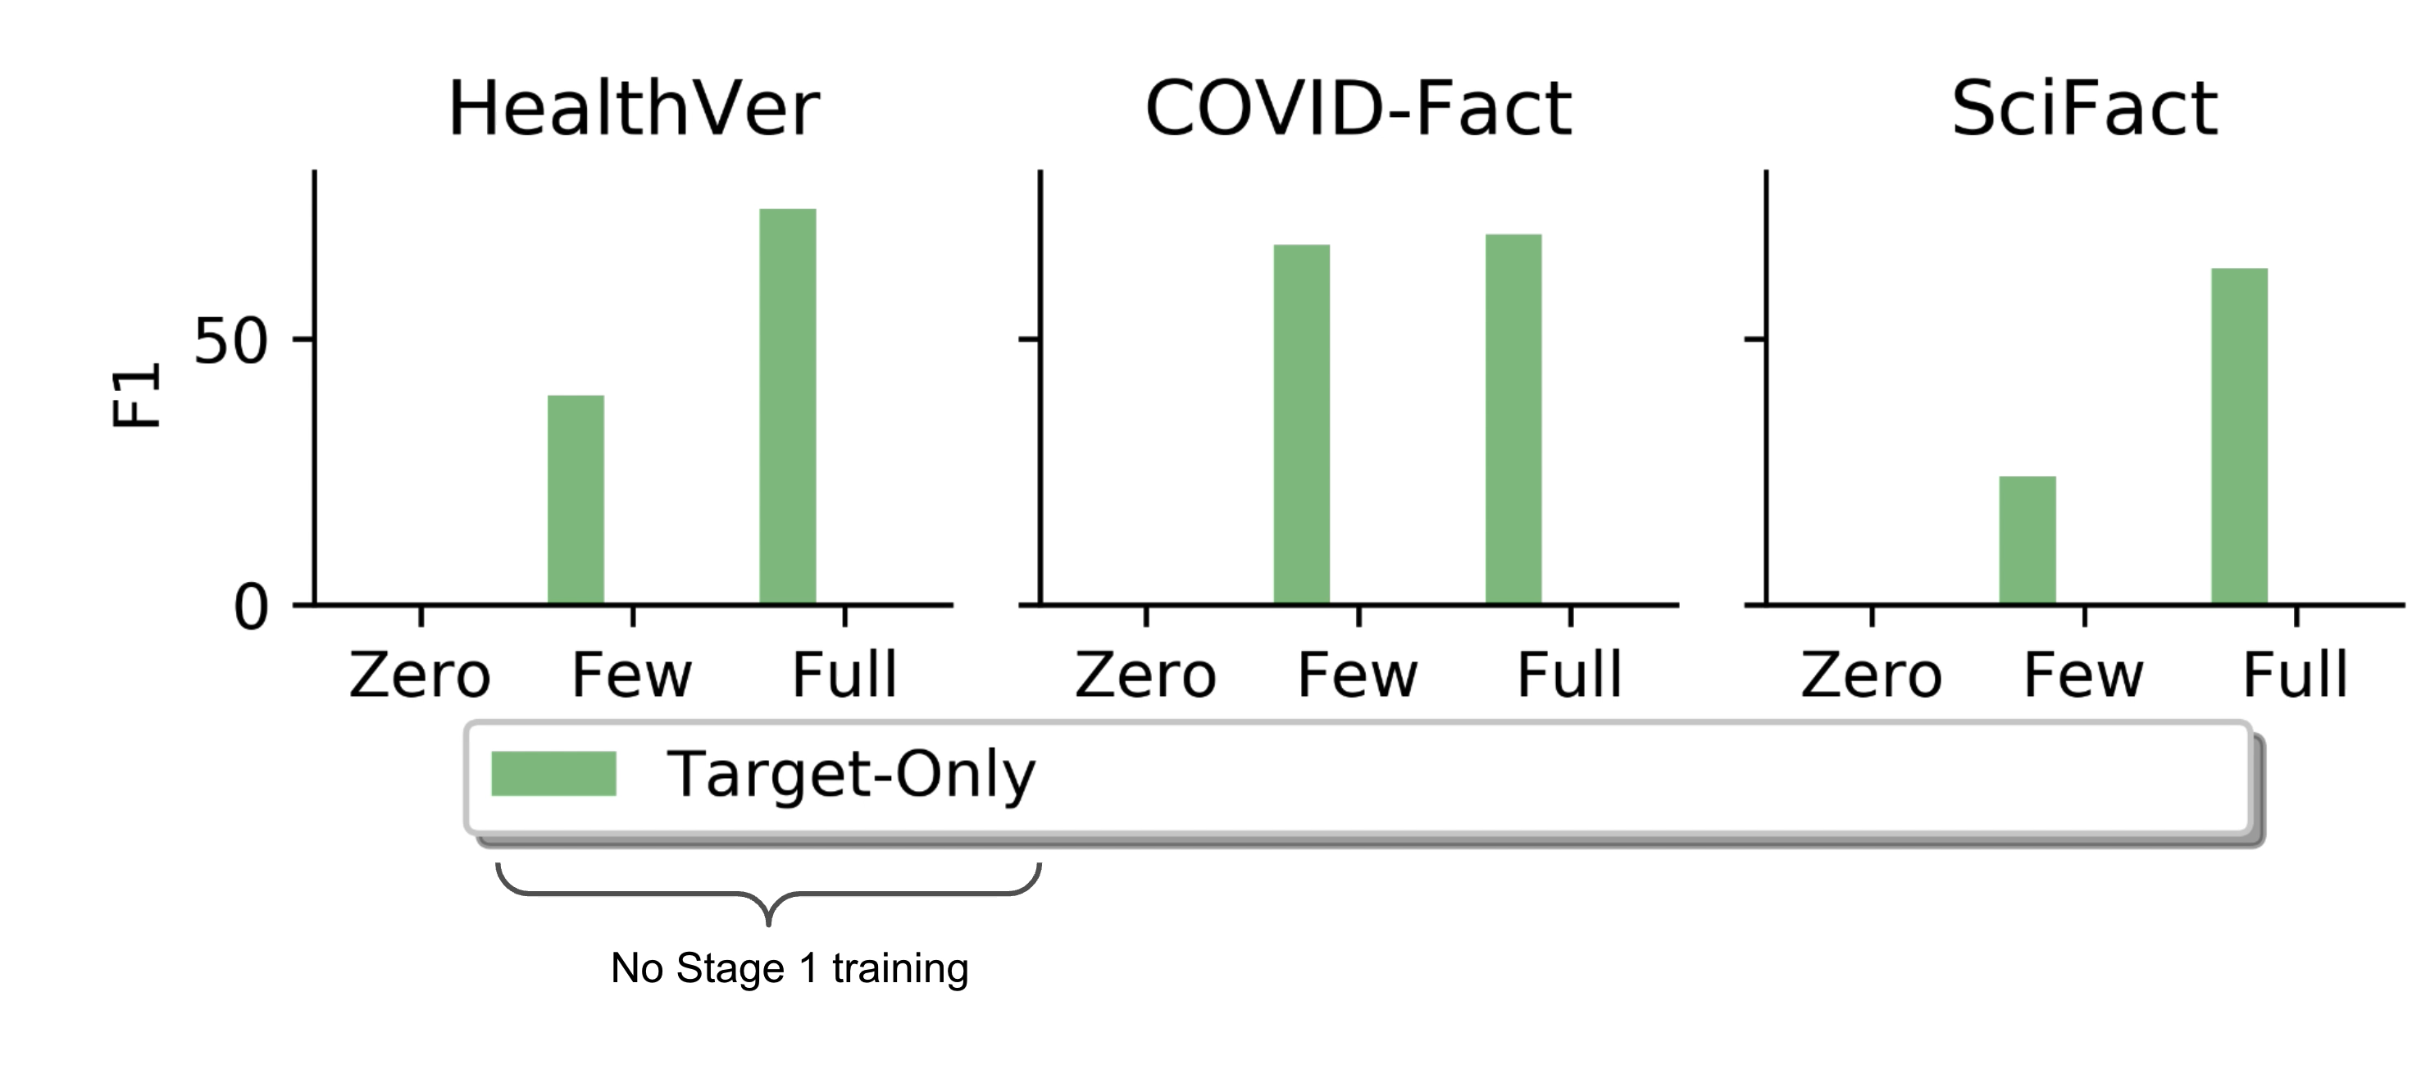
\includegraphics[width=1\textwidth]{Crop/Ablations_1.png}
        }
        \only<2> {
            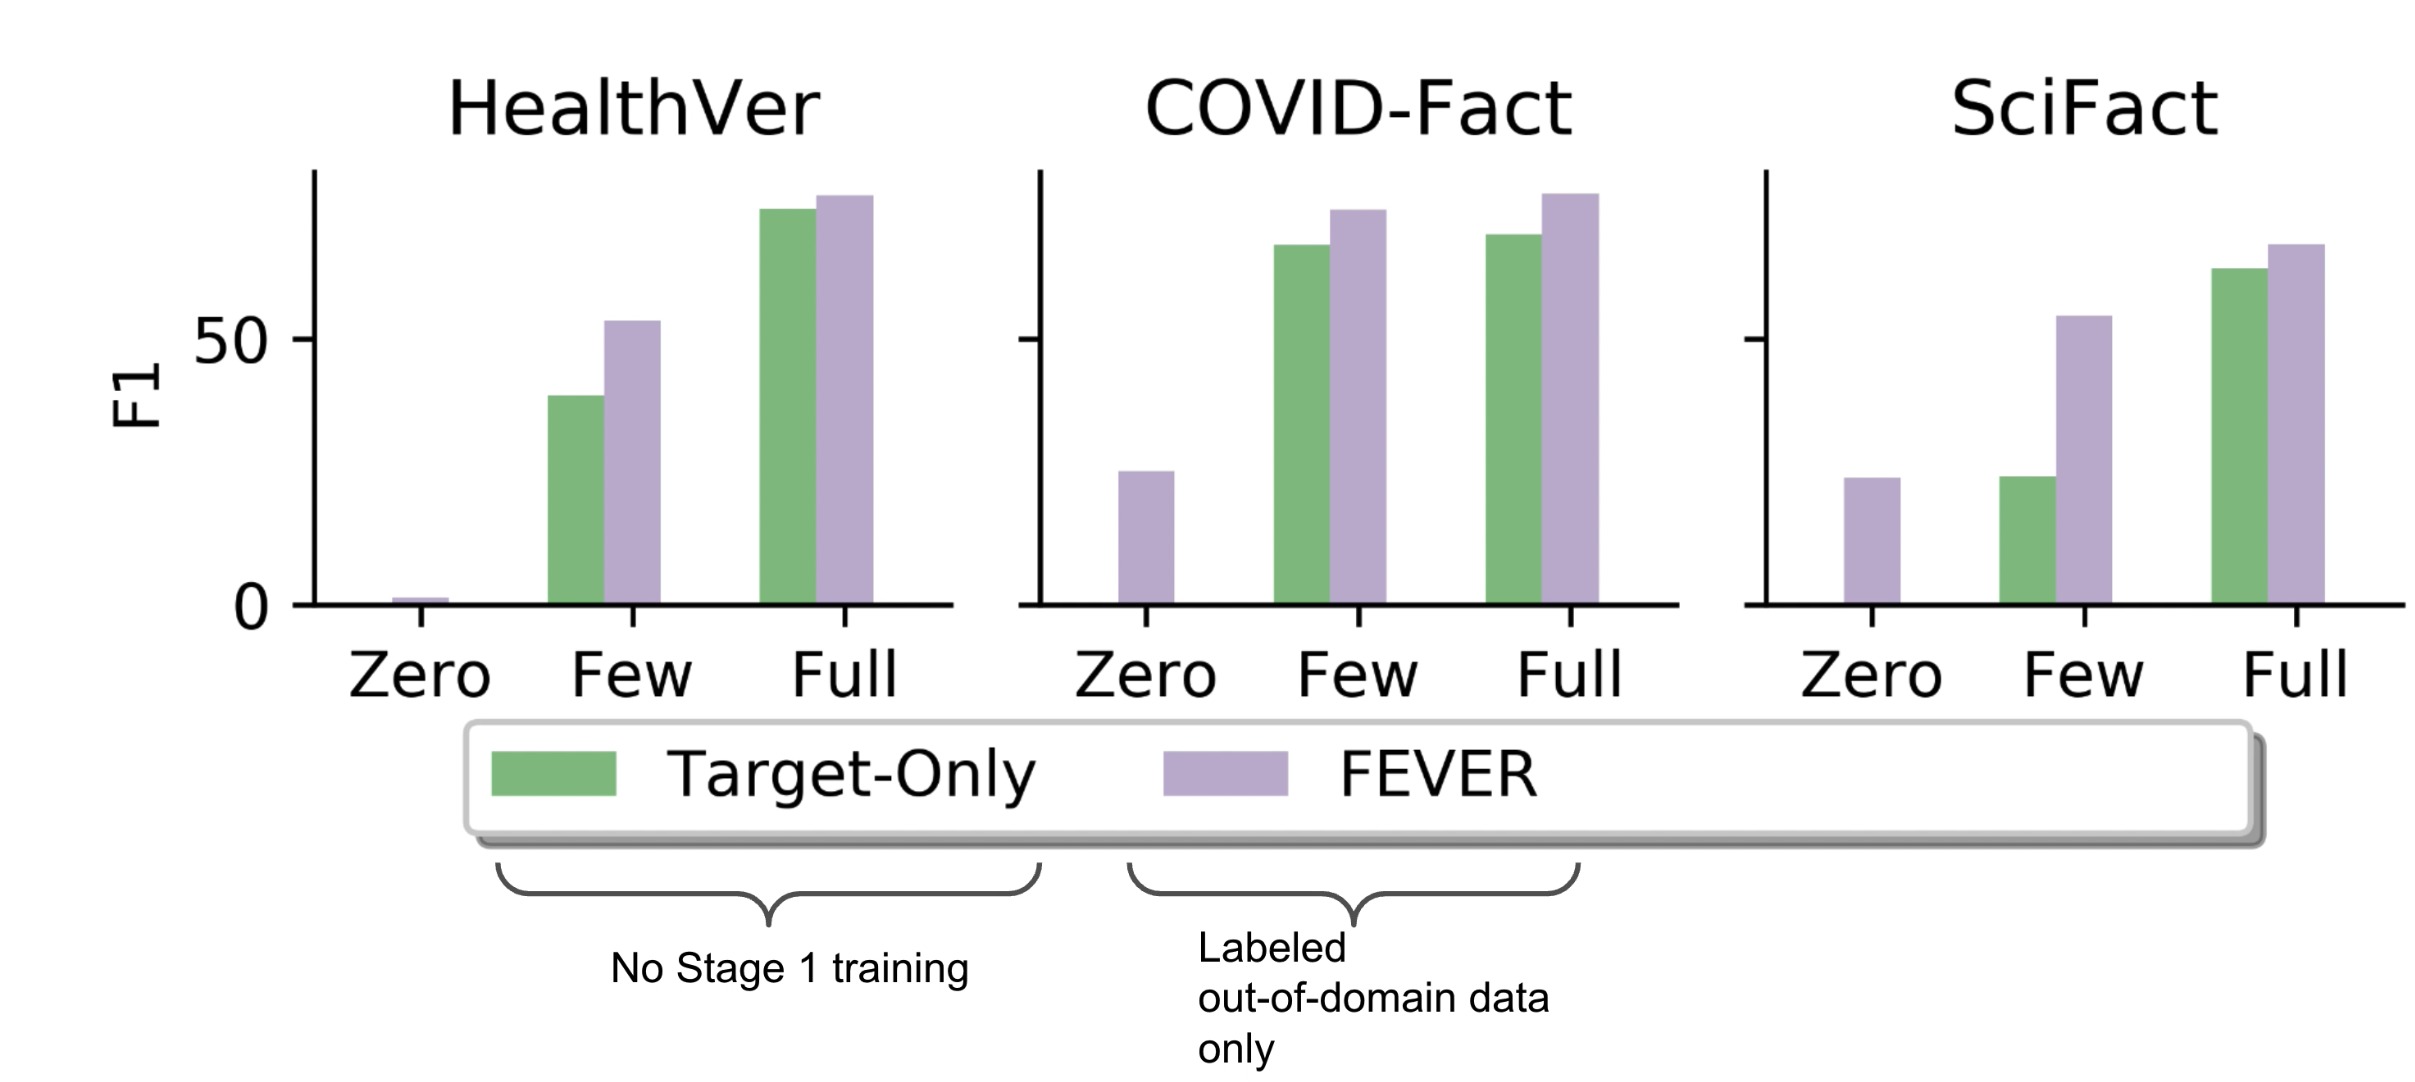
\includegraphics[width=1\textwidth]{Crop/Ablations_2.png}
        }
        \only<3-> {
            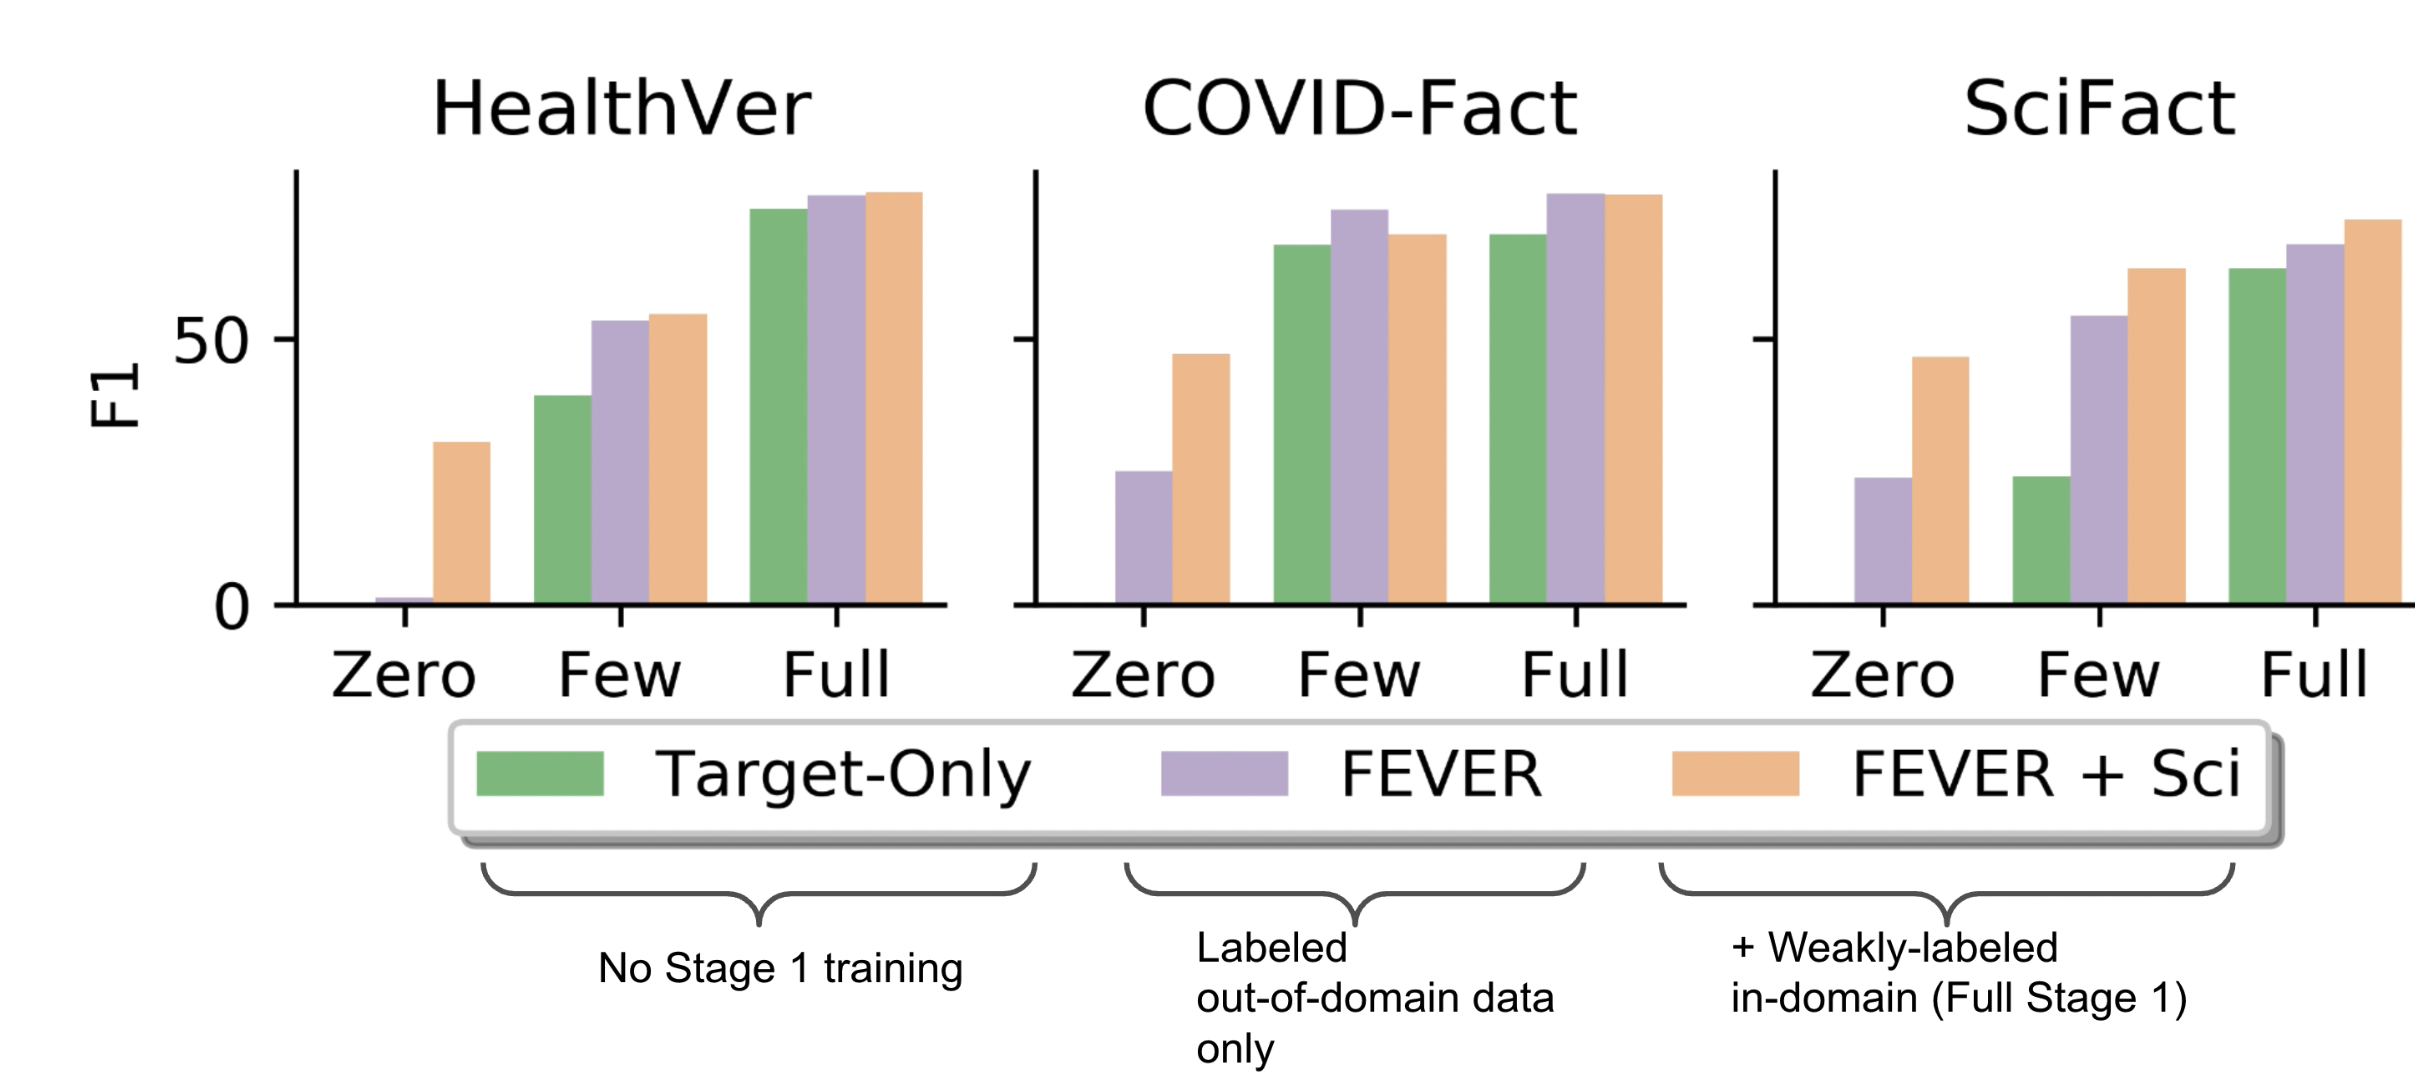
\includegraphics[width=1\textwidth]{Crop/Ablations_3.png}
        }

        \visible<4>{
            \begin{minipage}{0.65\textwidth}
                \begin{block}{}
                    Pretraining with weakly-supervised in-domain data improves few / zero shot performance.
                \end{block}
            \end{minipage}
        }

    
\end{frame}
%------------------------------------------------
 
 


                

\onehalfspacing
\begin{frame} % Use [allowframebreaks] to allow automatic splitting across slides if the content is too long
	\frametitle{Reference}
	
	\begin{thebibliography}{99} % Beamer does not support BibTeX so references must be inserted manually as below, you may need to use multiple columns and/or reduce the font size further if you have many references
		\footnotesize % Reduce the font size in the bibliography
		
		\bibitem[Stanford]{p1}
			\href{https://aclanthology.org/2022.findings-naacl.6}{MULTIVERS: Improving scientific claim verification with
            weak supervision and full-document context}
        \bibitem[Stanford]{p2}
        \href{https://aclanthology.org/2023.findings-acl.387.pdf}{Scientific Fact-Checking: A Survey of Resources and Approaches}
			\newblock Juraj Vladika and Florian Matthes
        \bibitem[Stanford]{p3} Longformer: The Long-Document Transformer
        \newblock Iz Beltagy, Matthew E. Peters and Arman Cohan
		
        \hspace{-1.9em}
\includegraphics[width=1.5em]{Icons/github.png}
        \textcolor{blue}{\href{https://github.com/dwadden/multivers}{Code and model checkpoints for the MultiVerS model}}
          \newblock \textcolor{black}{dwadden/multivers}
	\end{thebibliography}
\end{frame}



%	CLOSING SLIDE
%----------------------------------------------------------------------------------------

\begin{frame} % The optional argument 'plain' hides the headline and footline
	\begin{center}
		{\Huge Thanks for listening!}
		
		\bigskip\bigskip % Vertical whitespace
		
		{\LARGE Q\&A section}
	\end{center}
\end{frame}
%------------------------------------------------


\end{document}
